\documentclass[12pt]{scrartcl}
\usepackage[sexy]{evan}
\usepackage{graphicx}

\usepackage{answers}
\Newassociation{hint}{hintitem}{all-hints}
\renewcommand{\solutionextension}{out}
\renewenvironment{hintitem}[1]{\item[\bfseries #1.]}{}
\declaretheorem[style=thmbluebox,name={Theorem}]{thm}

 %Sets
\newcommand{\N}{\mathbb{N}}
\newcommand{\Z}{\mathbb{Z}}
\newcommand{\F}{\mathbb{F}}
\newcommand{\Q}{\mathbb{Q}}
\newcommand{\R}{\mathbb{R}}
\newcommand{\C}{\mathbb C}
\newcommand{\T}{\mathbb T}
\renewcommand{\hat}{\widehat}
\let \phi \varphi
\let \mc \mathcal
\let \ol \overline
%From Topology
\newcommand{\cT}{\mathcal{T}}
\newcommand{\cB}{\mathcal{B}}
\newcommand{\cC}{\mathcal{C}}
\newcommand{\cH}{\mathcal{H}}

\newcommand{\supp}{\text{supp }}

\newcommand{\aint}{\mathrel{\int\!\!\!\!\!\!-}}
\let \grad \nabla

\begin{document}
\title{Math 214}
\author{Vishal Raman}
\thispagestyle{empty}
$ $
\vfill
\begin{center}

\centerline{\huge \textbf{Math 214: Differentiable Manifolds} } 
\centerline{Professor: Richard Bamler, Spring 2021}
\centerline{Scribe: Vishal Raman}
\end{center}
\vfill
$ $
\newpage
\thispagestyle{empty}
\tableofcontents
\newpage
%\maketitle
\section{January 19th, 2021}
\subsection{Topology Review}
\begin{definition}[Topological Space] $(X, O_X \subset \mc P(X))$, where $A \in O_x$ are the open sets which satisfy the following:
\begin{enumerate}
\item $\emptyset, X \in O_X$.
\item $A, B \in O_X$ implies $A \cap B \in O_X$
\item $A_i \in O_X$, $i \in I$, then $\bigcup_{i \in I} A_i \in O_X$.
\end{enumerate}
We say that $A \subset X$ is closed if $X \setminus A$ is open.  $U \subset X$ is a neighborhood of $p \in X$ if $\exists A$ such that $p \in A \subset U$.
\end{definition}

\begin{example} Take a metric space $(X, d)$.  The topology is generated as follows: $A \subset X$ is open if $\forall p \in A$, $\exists r > 0$ such that $B_r(p) \subset A$.
\end{example}

\begin{definition}  $\mc B \subset \mc P(X)$ is called a \textbf{basis} for the topology on $X$ if for every subset $A \subset X$, $A$ is open if and only if $A$ is a union of elements of $\mc B$.
\end{definition}
\begin{example} For a Euclidean space, $\mc B = \{B_r(x) \subset \R^n: r \in \Q, r > 0, x \in \Q^n\}$ is a basis for the topology.  Note that this basis is countable, so $\R^n$ is 2nd countable.  
\end{example}

Let $(X, O_X)$, $(Y, O_Y)$ be topological spaces.  

\begin{definition} A function $\phi : X \to Y$ is continuous if for any open subset $B \subset Y$, $\phi^{-1}(B) \subset X$ is open.  
\end{definition}

\begin{definition} $\phi: X \to Y$ is a homeomorphism if it is a continuous bijection whose inverse is continuous.  
\end{definition}

\begin{definition} Let $Y \subset X$ a topological space.  We set $O_Y = \{A \cap Y : A \in O_X\}$.
\end{definition}

\begin{example}
The subspace topology is the coarsest topology so that the inclusion map $Y \to X$ is continuous(also called the initial topology).  
\end{example}
\begin{example} $\R \times \{0\} \subset \R^2$ has the same topology as $\R$.  In other words, it is clear that $\R \approx \R \times \{0\}$, where the approximate sign indicates a homeomorphism.
\end{example}

\begin{thm} (Topological Invariance of Dimension) If we take $\R^m, \R^n$ with open subsets $U \subset \R^m$ and $V \subset R^n$.  If we have $\phi: U \to V$ a homeomorphism, then we must have $m = n$.
\end{thm}
The proof is beyond the scope of the class, but uses homology groups.  

\begin{definition} Given a topological space $X$, $X$ is called locally Euclidean (of dimension $n$) at $p \in X$ if there is an open neighborhood about $p \in U \subset X$ that is homeomorphic to an open subset of $\R^n$.
\end{definition}

\begin{lemma} The $n$ is uniquely determined by $p$.  
\end{lemma}
\begin{proof} Assume that $X$ was locally Euclidean at $p$ of dimensions $n_1, n_2$.  There are neighborhoods $p \in U_i \subset X$ and homeomorphisms $\phi_i : U_i \to \hat{U_i} \subset \R^{n_i}$.  Consider the image of $U_1 \cap U_2$ under both homeomorphisms.  If we take $\phi_2 \circ \phi_1^{-1}: \phi(U_1 \cap U_2) \to \phi_2(U_1 \cap U_2)$, a homeomorphism, so it follows that $n_1 = n_2$ by Topological Invariance of Dimension.
\end{proof}

\begin{definition} A space $X$ is \textbf{Hausdorff} if for any $p, q \in X$, $p \ne q$ there exists open subsets $U, V$ with $p \in U$, $q \in V$ so that $U \cap V = \emptyset$.
\end{definition}

\begin{exercise} For any $p, q \in X$, if there is a separating continuous function $f: X \to \R$ such that $f(p) \ne f(q)$, then $X$ is Hausdorff.
\end{exercise}

\begin{definition} $K \subset X$ is compact if every open cover of $K$ has a finite subcover.  
\end{definition}

Some useful facts, a subspace of a Hausdorff space is Hausdorff, Hausdorff + Compact implies Closed, $\phi: X \to Y$ continuous, $K$ is compact, then $\phi(K)$ is compact.  We can use these to show that for $\phi: X \to Y$ with $X$ compact, $Y$ Hausdorff with $\phi$ continuous, bijective, then $\phi$ is a homeomorphism.  
\subsection{Smooth Manifolds}
\begin{definition} A topological space $M$ is called an $n$-dimensional \textbf{topological manifold} if $M$ satisfies the following:
\begin{itemize}
\item $M$ is locally Euclidean at any point,
\item $M$ is Hausdorff,
\item $M$ is second countable.
\end{itemize}
\end{definition}

\begin{example}[Manifold - Hausdorff] Suppose we drop the Hausdorff condition.  Take $X = (\R \times \{0, 1\}) \setminus \sim$, where  $(x, 0) \sim (x, 1)$ if $x < 0$.  Consider the quotient map $\pi: \R\times\{0, 1\} \to X$.  Call $A \subset X$ open iff $\pi^{-1}(A)$ is open.  Each branch of the line are open subsets, each homeomorphic to $\R$.  
\end{example}

\begin{example}[Manifold - Second Countable] Take an uncountable subset $S$ equipped with the discrete topology.  Set $X = S \times \R$.  

A more interesting example called the "long line" is as follows: 
\begin{lemma} There is an uncountable, well-ordered set $S$ such that $S$ has a maximal element $\Omega \in S$ and for all $\alpha \in S$, $\alpha \ne \Omega$, the set $\{x \in S| x < \alpha\}$ is countable.  
\end{lemma}
Now, set $X = (-\infty, 0) \cup S \times [0, 1)$ under the lexicographic ordering.  This turns out to be Hausdorff and locally Euclidean but not second countable.  
\end{example}

\begin{exercise} If $M$ is $0$-dimensional topological manifold , then $M$ is a finite or countable set equipped with the discrete topology.  
\end{exercise}
\begin{exercise} If $M^n$ is a top. manifold and $M' \subset M^n$ is open, then $M'$ is an $n$-dimensional top. manifold.  
\end{exercise}
\begin{example} Take $S^1 \subset \R^2$, a circle.  This is a 1-dimensional topological manifold.    
\begin{itemize}
\item It is easy to show that $S^1$ is Hausdorff and second countable.
\item Define $U_i^+ = \{(x_1, x_2) \in S^1 | x_i > 0\}.$  We similarly define $U_i^-$.  Then $S^1$ is the union of all the intervals.  We can construct the map $\phi_i^+ : U_i^+ \to (-1, 1)$ by projecting onto the corresponding axis.  This is a homeomorphism.  
\end{itemize}
\end{example}

\pagebreak
\section{January 21st, 2021}
\subsection{Coordinate Charts}
\begin{definition} A \textbf{coordinate chart} on $M$ is a pair $(U, \phi)$ where $U\subset M$ is open and $\phi: U \to \hat{U} $ is a homeomorphism to an open subset $\hat{U} \subset \R^n$.
\end{definition}

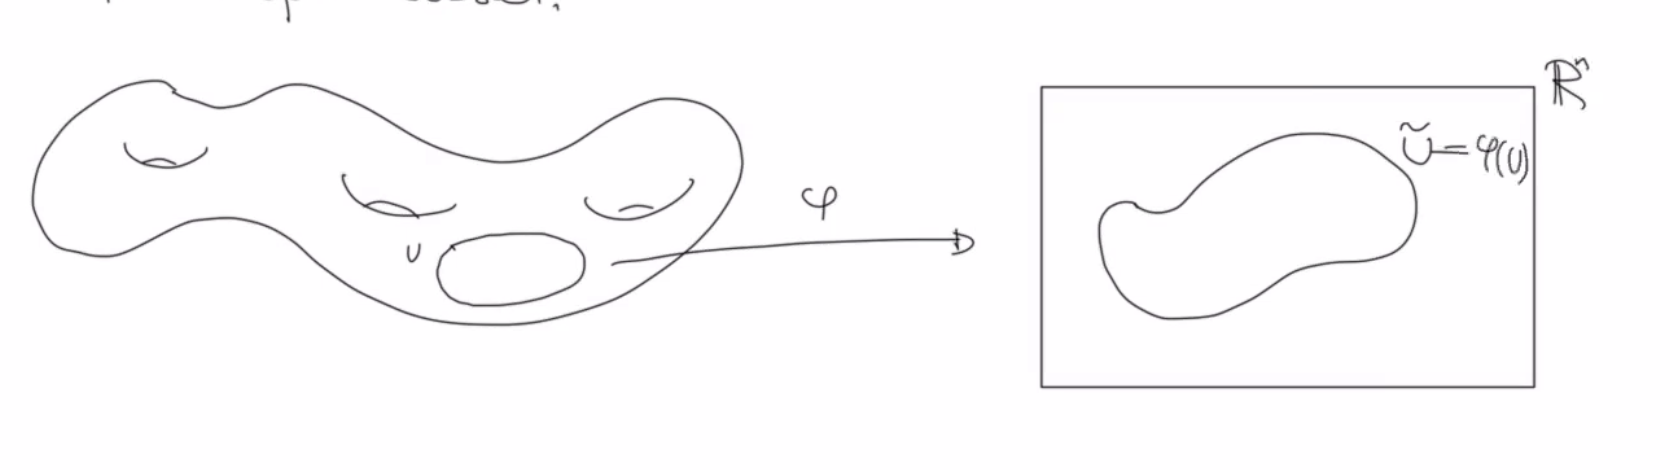
\includegraphics[scale=0.5]{chart.png}
\begin{remark} We can actually drop the condition that $\hat{U}$ is open, but the proof of this requires the notion of homology.

We will often write $\phi(p) = (\phi^1(p), \phi^2(p), \dots, \phi^n(p))$, which are local coordinates.  A way to think about a coordinate chart is just a set of scalar functions, which are the coordinate functions.  
\end{remark}

\begin{thm} Take $V \subset \R^n$ open, $F: V \to \R^k$ continuous.  We claim the graph $$\Gamma(F) = \{(x, F(x)): x \in \R^n\} \subset \R^{n+k}$$ is a manifold. 
\end{thm}
\begin{proof}
Take $(\Gamma(F), \phi)$, where $\phi$ is the projection of the graph onto $\R^n$.   It is clear that $\Gamma(F) \cong V$.
\end{proof}

\begin{example} Take $S^n = \{x \in \R^{n+1 : |x| = 1} \subset \R^{n+1}\}$.  We claim this is a manifold.  

Define $U_i^+ = \{(x^1, \dots, x^{n+1}) : x_i > 0\}$. Similarly define $U_i^-$.  It is clear that $M$ is the union of all the $U_i^+$'s and $U_i^-$'s.  Note that $U_i^{\pm}$ is the graph of the map from $B^n(0, 1) \to \R$ given by $y \mapsto \pm \sqrt{1 - |y|^2}.$  It follows that $S^n$ is a topological manifold.
\end{example}

\begin{example}[Projective Space]  We define $\R P^n = (\R^{n+1} \setminus \{0\})/ \sim$, where the equivalence relation is defined by $x \sim y$ if $x = \lambda y$ for some $\lambda \ne 0$.  We can also view this as a set of lines through the origin.  The quotient space is equipped with a projection map $\pi: \R^{n+1}\setminus \{0\} \to \R P^n$.  We can then use the Quotient topology: $A \subset \R P^n$ is open if $\pi^{-1}(A)$ is open.  

We write $[(x_1, \dots, x^{n+1})] = [x^1 : \dots : x^{n+1}]$.  One should check that $\R P^n$ is Hausdorff and second countable. We show that $\R P^n$ is locally Euclidean.  

Define $U_i^* = \{x \in \R^{n+1} \setminus \{0\} : x_i \ne 0\}$ and let $U_i = \pi(U_i^*)$.  Note that 
$$U_i = \{[x^1 : \dots : x^{n+1}] : x^i \ne 0\} = \{[\frac{x^1}{x^i} : \dots : 1 : \frac{x^{n+1}}{x^i}]: x^i \ne 0\}$$
and furthermore
$$U_i = \{[x^1 : \dots : 1 : \dots : x^{n+1}]\}.$$

If we define $\phi_i^* : U_i^* \to \R^n$ given by $(x^1, \dots, x^{n+1}) \mapsto \left (\frac{x^1}{x^i}, \dots, \frac{x^{n+1}}{x^i}\right )$.

We claim that there exists a continuous map $\phi_i: U_i \to \R^n$ so that the corresponding commutative diagram commutes: this is just the natural map associated to the quotient.  

Furthermore, $\phi_i$ is a homeomorphism with inverse $(x^1, \dots, \hat{x^i}, \dots, x^{n+1}) \mapsto [x^1 : \dots : 1 : \dots : x^{n+1}].$
\end{example}
\subsection{Connectivity}
Given a topological space $X$, we have the following definitions:
\begin{definition} $X$ is connected if the only subsets that are open and closed are $\emptyset, X$.
\end{definition}
\begin{definition} A space is path-connected if for any $p, q \in X$ there is a continuous path between them.  
\end{definition}
\begin{thm} If $M^n$ is a topological manifold, $M$ is connected if and only if $M$ is path connected.  
 \end{thm}
 \begin{proof}
 It suffices to show the forward direction.  The proof is the same in the case of open subsets of $\R^n$.  
 \end{proof}
 
\subsection{Local Compactness and Paracompactness}

\begin{proposition} Given $M^n$, for all $p \in M$, there exists a compact neighborhood i.e. $M$ is locally compact.
\end{proposition}
Let $X$ be a topological space.
\begin{definition} An exhaustion by compact subsets is an increasing sequence of subsets $K_1 \subset K_2 \subset \dots \subset X$ such that $K_i$ is compact and $K_i \subset \text{Int}(K_{i+1})$ and $\bigcup_i K_i = X$.
\end{definition}

\begin{remark} This also implies that $X = \bigcup_i \text{Int}(K_i)$.  If $K^i \subset X$ is some other compact subset,  there is some $j$ such that $K^i \subset \text{Int}(K_j)$.
\end{remark}
\begin{proposition} If $X$ is second countable, and locally compact, Hausdorff, then $X$ has an exhaustion by compact subsets.  
\end{proposition}
\begin{proof} First, take $\mc B$ a countable basis for the topology of $X$.  Take $\mc B' = \{B \in \mc B : \ol{B} \text{ compact}\}$, which is still a basis for the topology.  Call these sets $\{U_1, U_2, \dots \}$.  Choose $K_1 = \ol{U_1}$.  For $K_2$, cover $K_1$ with possibly several $U_i$ such that $K_1 \subset U_1 \cup \dots \cup U_{m_2}$ so that $K_2 = \overline{U_1} \cup \dots \cup \ol{U_{m_2}}$, which is compact.  We continue this process to form an exhaustion. 
\end{proof}

\begin{definition} Take $\mc U \subset \mc P(X)$.  This is a cover of $X$ if $X = \bigcup_{U \in \mc U} U$.  A collection is called locally finite if every $p \in X$ has a neighborhood $p \in W \subset X$ such that $W$ only intersects finitely many $U \in \mc U$.    
\end{definition}

\begin{definition} A collection of subsets $\mc V$ is called a refinement of some other collection $\mc U$ if for every $V \in \mc V$ there is $U \in \mc U$ such that $V \subset U$.  
\end{definition}

\begin{definition} $X$ is called paracompact if every open cover has a locally finite refinement. 
\end{definition}
\begin{thm} Every topological manifold is paracompact.  
\end{thm}
\pagebreak
\section{January 26th, 2021}
\subsection{Smooth Structures}
\begin{definition} Let $M^n$ be a topological manifold.  Two charts $(U, \phi), (V, \psi)$ of $M$ have a transition map: $\psi \circ \phi^{-1}$.  This map is a homeomorphism.
\end{definition}
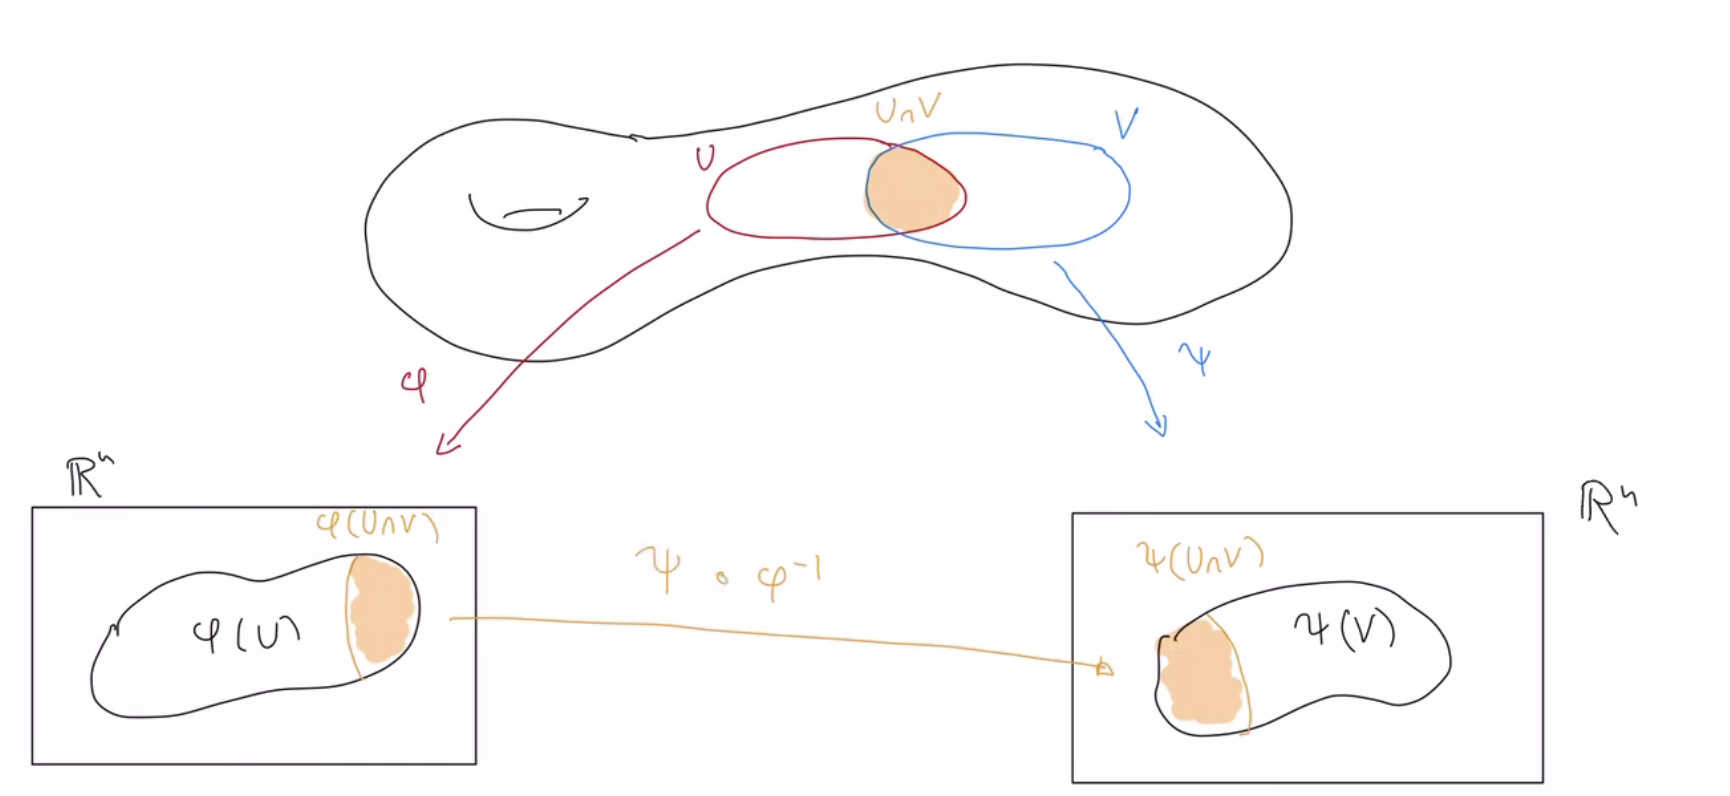
\includegraphics[scale=0.5]{transition}
\begin{definition} Two charts are smoothly compatible if the transition maps in both directions are smooth.
\end{definition}
\begin{definition} An atlas $\mc A$ of $M$ is a collection of charts such that the domains of the charts cover $M$.  An atlas $\mc A$ is smooth if any two charts in $\mc A$ are smoothly compatible.  An atlas $\mc A$ is called a maximal smooth atlas on $M$ if there is no smooth atlas containing $\mc A'$ that contains $\mc A$.  
\end{definition}
\begin{theorem}
Every smooth atlas $\mc A$ of $M$ is contained in a unique maximal smooth atlas.  
\end{theorem}
\begin{proof}
We first address the existence of a a maximal atlas $\ol{\mc A}$.  We define 
$$\ol{\mc A} = \{(U, \phi) : (U, \phi) \text{ is compatible with all } (V, \psi) \in \mc A \}.$$
$\mc A \subset \ol{\mc A}$ is clearly an atlas so it suffices to show that it is smooth.  

Take $(U_1, \phi_1)$, $(U_2, \phi_2) \in \ol{\mc A}$.  We check that $\phi_2 \circ \phi_1^{-1}(U_1 \cap U_2)$ are smooth.   Take some $q \in \phi_1(U_1 \cap U_2)$ so that $q = \phi_1(p)$ for $p \in U_1 \cap U_2$.  Choose $(V, \psi)$ so that $p \in V$.  Then,
 $$\phi_2 \circ \phi_1^{-1} \vert_{\phi_1(U_1 \cap U_2 \cap V)} = (\phi_2 \circ \psi^{-1}\vert_{\psi(U_1 \cap U_2 \cap V)}) \circ (\psi \circ \phi_1^{-1}\vert_{\psi(U_1 \cap U_2 \cap V)}).$$
\end{proof}
\begin{remark} If $(U_1, \phi_1) \in \mc A_1$ is smoothly compatible with any chart $(U_2, \phi_2) \in \mc A_2$, then $\ol{\mc A_1} = \ol{\mc A_2}$.
\end{remark}
\begin{definition} A maximal smooth atlas $\mc A$ on a topological manifold $M$ is called a smooth structure on $M$.
\end{definition}
\begin{definition} A smooth manifold is a pair $(M^n, \mc A)$, where $M^n$ is a topological manifold and $\mc A$ is a smooth structure.  
\end{definition}
Some exercises:
\begin{itemize}
\item If $(U, \phi) \in \mc A$ and $U' \subset U$ open, then $(U', \phi\vert_{U'}) \in \mc A$.
\item If $(U, \phi) \in \mc A$ and a diffeomorphism $\psi: \phi(Y) \to \psi(\phi(U)) \subset \R^n $, then $U(\psi \circ \phi) \in \mc A$.
\item If $\phi: U \to \R^n$ is injective has the property that for any $p \in U$, there is an open neighborhood $p \in U_p \subset U$ such that $(U_p, \phi \vert_{U_p})\in \mc A$, then $(U, \phi) \in \mc A$.
\end{itemize}
\subsection{Examples of Smooth Structures}
\begin{itemize}
\item Take $\R^n$.  Choose a maximal atlas containing $\{(\R^n, \text{id}_{\R^n})\}$.  
\item  Given $(M^n, \mc A)$ a smooth manifold, $M' \subset M$ open, take $\mc A' = \{(U, \phi) \in \mc A | U \in M'\}$.  
\item Take a vector space $V$ with dimension $n$.  Take $$\mc A' = \{(V, \phi) : \phi: V \to \R^n \text{ linear isomorphisms}\}.$$
We take the maximal atlas containing $\mc A'$.
\item Take $M = \R$.  Define $\mc A$ to be the maximal atlas containing $(\R, \text{id}_\R)$.  We could also choose $\mc A^*$ to be the maximal atlas containing $(\R, \phi)$ where $\phi: \R \to \R$ is given by $x \mapsto x^3$.  These two structures are not the same, but the two charts are diffeomorphic.  
\end{itemize}
Does every topological manifold have a smooth structure?  For $n \le 3$, YES and unique up to diffeomorphism.  For $n > 4$, NO and if they do exist, they may not be unique.  Are there exotic spheres?
\pagebreak
\section{January 28th, 2021}
\subsection{Construction of Smooth Manifolds}
\begin{lemma} Let $M$ be an uncountable set of points and $\{(U_\alpha, \phi_\alpha)\}_{\alpha \in I}$, where $\phi_\alpha: U_\alpha \to \R^n$ are injective.  Assume that (1) $\phi_\alpha(U_\alpha \cap U_\beta) \subset \R^n$ open for all $\alpha, \beta\in I$ and (2) $\phi_\alpha \circ \phi_\beta^{-1}$ is smooth for all $\alpha, \beta \in I$, (3) $M$ is covered by countably many $U_\alpha$, (4) for all $p, q \in M$, $p \ne q$, there is a $\alpha \in I$ such that $p, q \in U_\alpha$ or $\alpha, \beta \in I$ such that $p \in U_\alpha, q \in U_\beta$.

Then, $M$ has a unique topology and smooth structure such that $(U_\alpha, \phi_\alpha)$ are smooth charts.
\end{lemma}
\begin{proof}
We define the topology by $A \subset M$ is open whenever $\phi_\alpha(A \cup U_\alpha) \subset \R^n$ is open for all $\alpha \in I$.  We take the smooth structure to be the maximum atlas containing the charts.
\end{proof}
\subsection{Grassmannian Manifolds}
\begin{definition} For $1 \le k \le n$, define $\text{Gr}_k(\R^n) = \{V \subset \R^n | \dim V = k\}$.  
\end{definition}
Note that $\text{Gr}_1(\R^n) =  RP^{n-1}$.

We construct topological and smooth manifolds on $\text{Gr}_k(\R^n)$.  Define $I = \{(P, Q), P, Q \subset \R^n, V = P \oplus Q, \dim P = k, \dim Q = n+k\}.$

For a given $(P, Q) = \alpha$ define $U_\alpha = \{V \in \text{Gr}_k(\R^n) | V \cap Q = \{0\}\}.$
\begin{lemma} For $V \in U_\alpha$, there is a unique linear map $A_{P, Q, V}: P \to Q$ such that $V = \{x + A_{P, Q, V}x \in P \oplus Q | x \in P\}$.  

This defines a map $\phi_\alpha: U_\alpha \to \text{Hom}(P, Q) \cong \R^{kx(n-k)}$.
\end{lemma}
\subsection{Manifolds with Boundary}
We have a manifold $M$ with a boundary $\partial M$.  

We denote $H^n = \{x^n \ge 0\} \subset \R^n$, the upper half space, the most basic example.  Note that $\partial H^n = \{x^n = 0\} \cong \R^{n-1}$.  The interior $\text{Int }H^n = \{x^n > 0\}$.  
\begin{definition} A topological manifold with boundary $M^n$ is a topological space such that is Hausdorff,
 second countable, and every point $p \in H^n$ has an open neighborhood $p \in U \subset M$ that is
  homeomorphic to some (relatively) open subset $\hat{U} \subset H$.
\end{definition}

\begin{remark} For $M$ a topological manifold, we have a topological manifold with boundary, $p \in M$ is interior if it has an open neighborhood homeomorphic to $\hat{U} \subset \R^n$ and a boundary point, if there is a chart $(U, \phi)$ such that $\phi(p) \in \partial H^n$.
\end{remark}
\begin{theorem}[Boundary Invariance] $M^n = \int M \cup \partial M$, and $\partial M$ is a topological $(n-1)$ manifold.
\end{theorem}
Note that the interior and boundary do not correspond to the topological notions of boundary and interior.  For example, take $M = \{x^n > 0\} \subset \R^n$, this has a topological boundary in $\R^n$ but no manifold boundary.  For any manifold with boundary $M$, the topological boundary of $M$ is empty and the topological interior within $M$ is $M$.

If we take $M = S^n \subset \R^{n+1}$, then $\partial M = \emptyset$ but the topological boundary is simply $S^n$.

\begin{remark} $\partial M$ is a manifold(without boundary).
\end{remark}

\subsection{Smooth Maps}
\begin{definition} $f: M \to \R^m$ is smooth if for every $p \in M$, there is a smooth chart $(U, \phi)$, $\hat{U} = \phi(U)$ such that $p \in U$ and $\hat{f} = f \circ \phi^{-1}: \hat{U} \to \R^n$. 
\end{definition}
We denote $C^\infty(M) : \{f: M \to \R^m \text{ smooth}\}$.
\end{document}
